\section{Introduction}

The field of connectomics is concerned with reconstructing the wiring diagram of the brain at nanometer resolutions. 
Recent advancements in image acquisition using multi-beam serial-section electron microscopy (sSEM) has allowed neuroscientists to produce terabytes of electron micrsocopy (EM) image data every hour~\cite{hildebrand2017whole}.
Neuroscientists believe that reconstructing an entire mammilian brain at fine resolution will enable new insights into the workings of the brain~\cite{kasthuri2015saturated}. 
These observations will allow for new advancements in neuromedicine and artificial intelligence (CITE). 
Segmentation is part of this reconstruction process, assigning a unique label for every neuron in the EM image. 
It is not feasible for domain experts to manually segment the vast amount of 3-D image data to model an entire brain.

A significant amount of research focuses on automatic reconstruction of the neurons in EM images because of the scope and importance of the problem~\cite{seymour2016rhoananet,nunez2014graph,parag2017anisotropic,zlateski2015image}.%TODO DOUBLE CHECL REFERENCES
All of these algorithms extract neuronal processes through the 3-D volumes using only the raw image data as input.
Oftentimes, convolutional neural networks (CNNs) predict membrane probabilities or affinities between voxels and apply simple thresholds to agglomerate the voxels into clusters~\cite{lee2015recursive,ronneberger2015u}.
These \textit{per-voxel} algorithms produce excellent results but currently fall short of complete reconstructions with error rates of approximately $X\%$. %TODO ADD ERROR RATES 

\begin{figure}
	\centering
	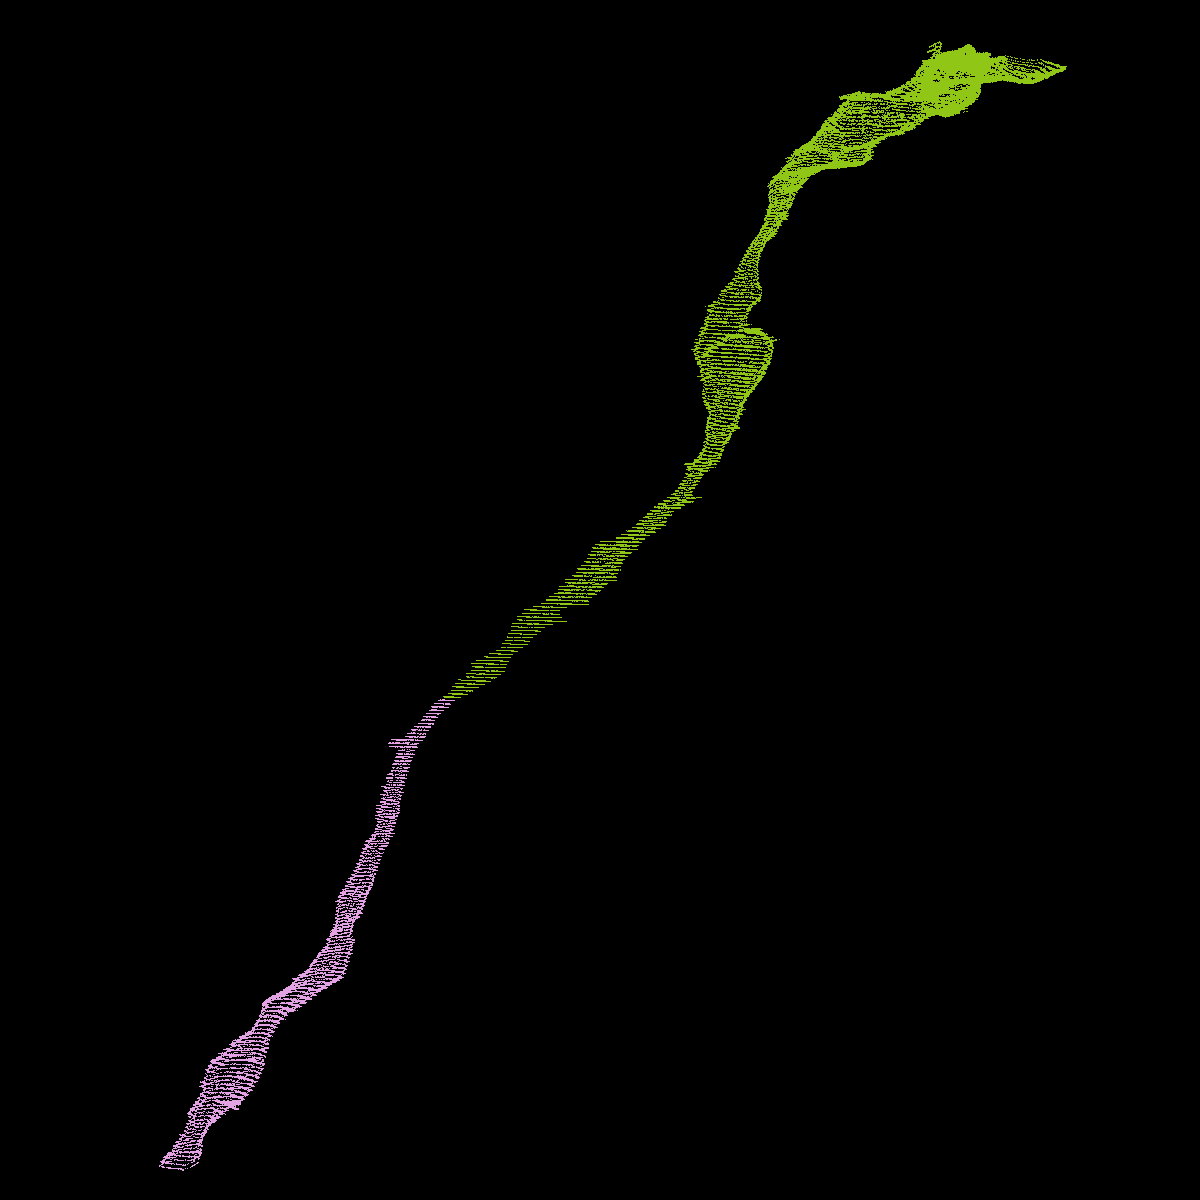
\includegraphics[width=0.42\linewidth]{./figures/merge_candidate1.png}
	\hspace{0.085\linewidth}
	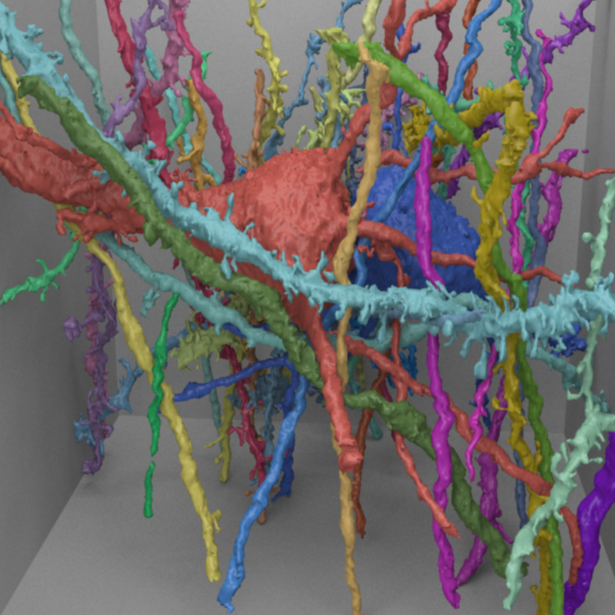
\includegraphics[width=0.42\linewidth]{./figures/intro-cube.png}
	\caption{We use 3D skeletons to combine neuron labels to full reconstructions. (TODO: Add schematic figure showing the difference between voxel-based / super-voxel based / graph-based algorithms with connections and hierarchy)} %TODO: SCHEMATIC FIGURE
\end{figure}

Researches currently address the failures of the per-voxel algorithms by training random-forest classifiers to agglomerate an oversegmentation of voxels~\cite{nunez2014graph} (CITE NEUROPROOF). 
These classifiers take the output of the per-voxel algorithms as input and generate high-level statistics such as affinity distributions between pixel regions. 
Presently, these methods use hand-designed features despite the evidence that machine-learned features perform better~\cite{bogovic2013learned}. 
These \textit{per-supervoxel} algorithms outperform the per-voxel algorithms but still do not provide the accuracy needed for large scale reconstructions of the brain.
Additionally, these methods do not fully leverage the wealth of shape information available (e.g., it is well known that neurons angle at less than $30$ degrees (CITE)). %TODO ADD CITATION FOR NEURON SHAPES

Here we present a \textit{graph-based} strategy that builds on top of the outputs of per-supervoxel methods by taking neuronal shape properties into account. 
Similarly we take as input automatic segmentations. 
However, we focus on general neuron shapes, traversing through the label volumes to identify potential merge candidates. 
From these locations we extract machine-learned features and generate a probability that two label segments should be joined. 
We construct a graph representation of the input label volume. 
Using graph-based optimization strategies enables us to enforce global constraints that more closely match the underlying biology of the images.
Lastly, we apply a globally optimal algorithm to produce a better reconstruction.

